\subsection{Динамика манипулятора}\label{part_dynamics}

\subsubsection{Общие замечания}
Введем в рассмотрение барицентрические СК $Ox_{ci}y_{ci}z_{ci}$\lefteqn,\footnote{Системы координат, чьи начала совпадают с центрами масс соответствующих звеньев.} где $i=\overline{1,5}$, показанные на рисунке~\ref{img_mass_frames}.
Заметим, что каждая СК $Ox_{ci}y_{ci}z_{ci}$ сонаправлена с $Ox_iy_iz_i$.

\begin{figure}[h!]
	\centering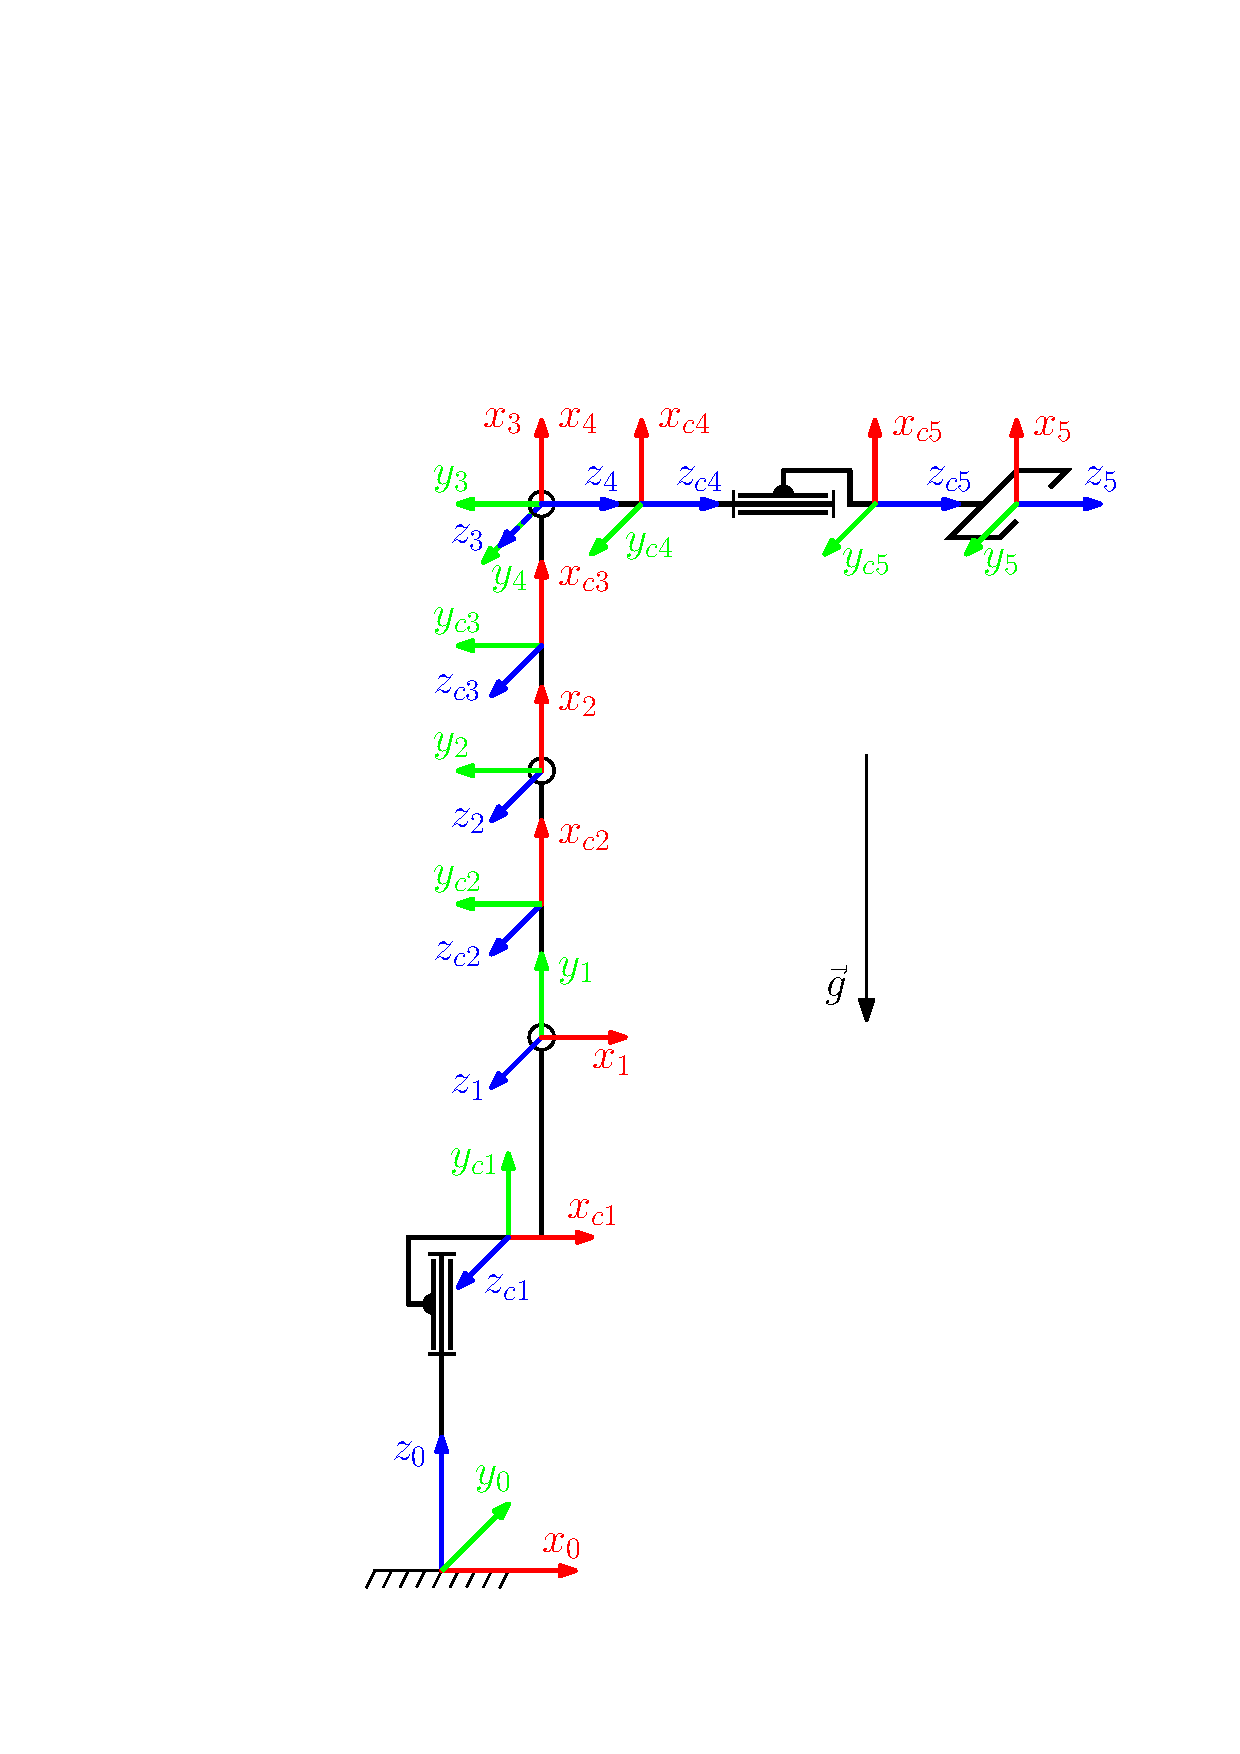
\includegraphics[height=16.5cm]{kinematics_mass_frames.pdf}
	\caption{Положение барицентрических СК и направление вектора $\vec{g}$.}
	\label{img_mass_frames}
\end{figure}

Для описания положения введенных СК воспользуемся следующими векторами:
\begin{equation}
    r^i_{i,\,ci} =
    \begin{bmatrix}
        x_{ci} \\ y_{ci} \\ z_{ci}
    \end{bmatrix}\!\!,\quad i = \overline{1,5},
\end{equation}
где $x_{ci}$, $y_{ci}$ и $z_{ci}$~--- некоторые постоянные величины.

Для компонент тензоров инерции $\mathcal{I}^{ci}_i = const$ введем следующие обозначения:
\begin{equation}
    \mathcal{I}^{ci}_i =
    \begin{bmatrix}
        I_{i,\,xx} & I_{i,\,xy} & I_{i,\,xz} \\
        I_{i,\,xy} & I_{i,\,yy} & I_{i,\,yz} \\
        I_{i,\,xz} & I_{i,\,yz} & I_{i,\,zz}
    \end{bmatrix}\!\!\ldotp
\end{equation}

Заметим, что
\begin{equation}
    g_0 =
    \begin{bmatrix}
        0 \\ 0 \\ -g
    \end{bmatrix}\!\!,
\end{equation}
где $g=9.82\text{ м}/\text{с}^2$.

В~заключении раздела приведем формулы для расчета величин, которые потребуются в дальнейшем (везде $i = \overline{1,5}$):
\begin{itemize}
    \item для расчета $r^0_{0,\,i}$ и ${}^{0}R_i$ (см.~Приложение~\ref{app_ht_matrices}):
        \begin{equation}
            {}^0A_i = {}^0A_1 \cdot {}^1A_2 \cdot \ldots \cdot {}^{i-1}A_i;
        \end{equation}
    \item для расчета $r^0_{0,\,ci}$:
        \begin{equation}
            \begin{bmatrix}
                r^0_{0,\,ci} \\ 1
            \end{bmatrix}
            = {}^0A_i
            \begin{bmatrix}
            r^i_{i,\,ci} \\ 1
            \end{bmatrix}\!\!;
        \end{equation}
    \item для расчета $r^i_{i-1,\,i}$:
        \begin{gather}
            {}^{i-1}A_i \quad \Rightarrow \quad {}^{i-1}R_i,\: r^{i-1}_{i-1,\,i},
            \\
            r^i_{i-1,\,i} = {}^{i-1}R_i^{-1} \!\cdot r^{i-1}_{i-1,\,i};
        \end{gather}
    \item для расчета $z^0_i$:
        \begin{equation}
            z^0_i = {}^{0}R_i \cdot z^i_i = {}^{0}R_i \cdot
            \begin{bmatrix}
                0 \\ 0 \\ 1
            \end{bmatrix}\!\!\ldotp
        \end{equation}
\end{itemize}

\newpage
